
\documentclass[11pt]{article}
\usepackage{amsmath}

\usepackage{url}
\usepackage{hyperref}
\usepackage{graphicx}
\usepackage{grffile}
\usepackage{xcolor}

\graphicspath{{figs/}}

\begin{document}

\title{Mathematics with the HP48G Calc}
\author{GNU Author}
\date{2006 February}
\maketitle

\section{Vector Algebra}
\subsection{Cross Product: Example 1}

A first basic example is given as follows:

\begin{align}
A &= \begin{bmatrix}
   2 \\
   2 \\
   3 \\
\end{bmatrix}
\end{align}

\begin{align}
B &= \begin{bmatrix}
   4 \\
   2 \\
   5 \\
\end{bmatrix}
\end{align}

You may search for the cross-product with  $ A \times B = C $
It gives:

\begin{align}
C &= \begin{bmatrix}
   4 \\
   2 \\
   -4 \\
\end{bmatrix}
\end{align}


\begin{itemize}
\item Example (1) using the HP48G
\begin{itemize}
\item You may enter  $ [ 2 \; 2 \; 3 ] $
\item You may enter  $ [ 4 \; 2  \; 5 ] $
\item In order to calculate the cross product, the "CROSS" function in the HP48G/HP50G will allow to give the solution:
\item The solution is:  $ [ 4 \;  2 \; -4 ] $
\end{itemize}
\end{itemize}




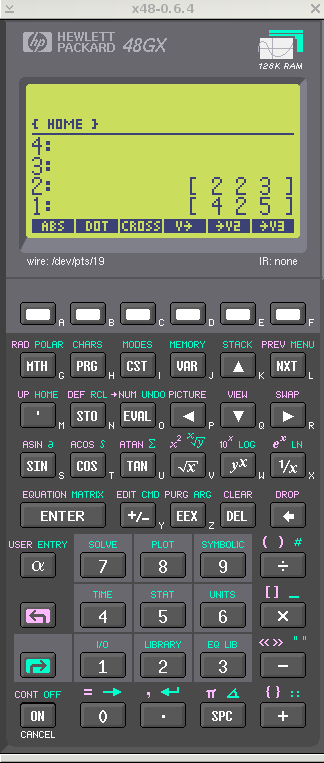
\includegraphics[scale,height=0.8\textheight]{20180422153058-cross-product02.png}

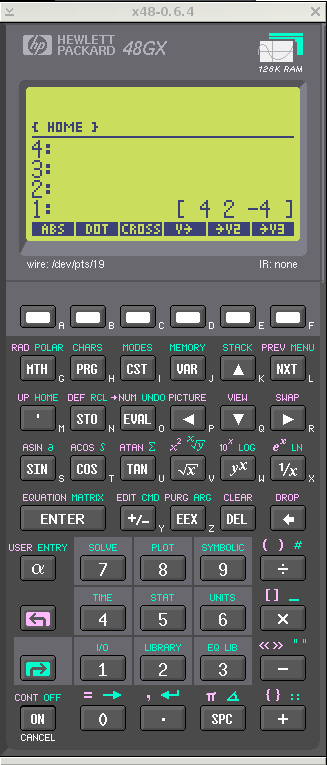
\includegraphics[scale,height=0.8\textheight]{20180422153111-cross-product02.png}


\begin{itemize}
\item Example (1) using nrpn:
\begin{itemize}
\item nrpn is a rapid method to check the results with little GNU spreadsheet.
\end{itemize}
\end{itemize}


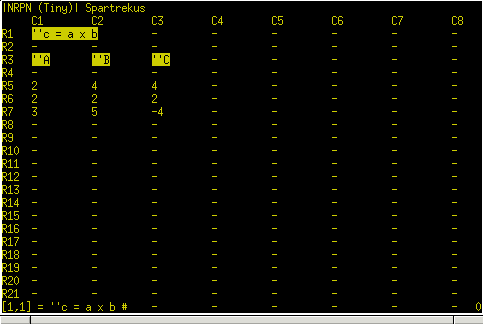
\includegraphics[scale,height=0.5\textheight]{20180422155226-cross-product02.png}

\end{document}
